\chapter{Prostate Cancer Detection Setting}

%% How the model is trained. Difference in architecture with "normal" VGG-16. Tiling, early stopping, optimizers.
\todo{Prostate cancer introduction}
RationAI trained and tested \emph{VGG-16}-based convolutional neural network on dataset provided by Masaryk Memorial institute. This chapter covers used data, model, model's training and achieved results.

\section{Dataset}

Dataset consist of Hematoxylin/Eosin stained WSI's, scanned using

What the dataset consists of, what is the data distribution, how it was collected. Origin of data.

\section{Gleason Patterns}

\section{Model and Training}

Utilized model is \emph{VGG-16} infused architecture, shown in Figure \ref{fig:rationai-vgg16} The model is trained training split of the dataset described in section PREV

\begin{figure}[!h]
    \begin{center}
    \begin{minipage}{0.75\textwidth}
      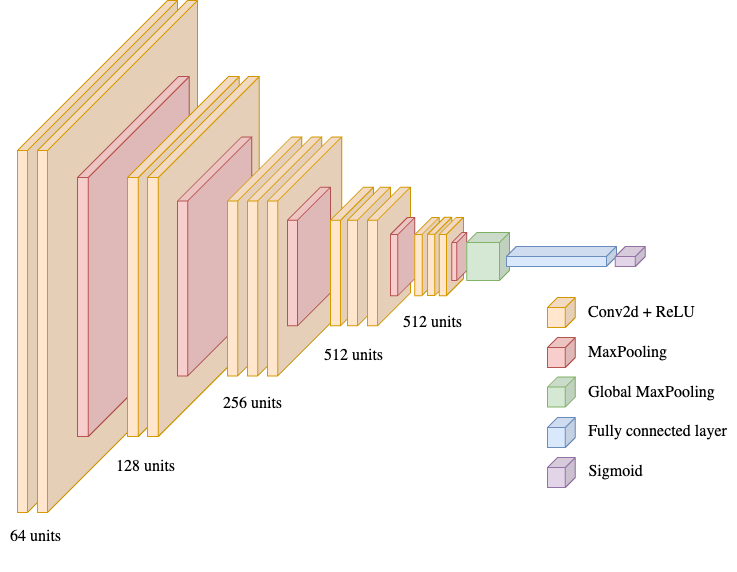
\includegraphics[width=\textwidth]{img/nn-arch.png}
    \end{minipage}
    \caption{Architecture of Prostate Cancer Binary Classifier model utilized by RationAI. Model is based on VGG-16, introduced by Simonyan and Zisserman in 2014 []. It differs in size of input image. Original VGG-16 model is trained to classify 1000 classes from ... dataset and utilizes 3 fully connected layers before applying softmax on the last one. In our solution, global max pooling is placed before single fully connected layer, reducing each of the 512 feature maps into one value. Sigmoid is applied to output of the fully connected layer, to turn its output into probabilistic distribution [].}
    \label{fig:rationai-vgg16}
    \end{center}

%% original vgg paper
%% how sigmoid makes it probability or whatever
\end{figure}

